%%%%%%%%%%%%%%%%%%%%%%%%%%%%%%%%%%%%%%%%%%%%%%%%%%%%%%%%%%%%%%%%%%%%%%%%%%%%%%

\documentclass{l3deliverable}

%%%%%%%%%%%%%%%%%%%%%%%%%%%%%%%%%%%%%%%%%%%%%%%%%%%%%%%%%%%%%%%%%%%%%%%%%%%%%%

\usepackage{graphicx}%
%

\version{Draft version

Made 31/10/2012~ by Team W}

\usepackage{tabularx}%
\usepackage{url}%
\usepackage{usecasedescription}%

%%%%%%%%%%%%%%%%%%%%%%%%%%%%%%%%%%%%%%%%%%%%%%%%%%%%%%%%%%%%%%%%%%%%%%%%%%%%%%
%% Check these macro values for appropriateness for your own document.

\title{Requirements Document}

\author{
    Gordon Reid: 1002536R\\
    Ryan Wells: 1002253W\\
    Kristopher Stewart: 1007175S\\
    David Selkirk: 1003646S\\
    James Gallagher: 0800899G\\
}

\date{1st November 2012}

\deliverableID{D3}
\project{PSD3 GE1 - Internship Management System}
\team{W}

%%%%%%%%%%%%%%%%%%%%%%%%%%%%%%%%%%%%%%%%%%%%%%%%%%%%%%%%%%%%%%%%%%%%%%%%%%%%%%

\begin{document}

%%%%%%%%%%%%%%%%%%%%%%%%%%%%%%%%%%%%%%%%%%%%%%%%%%%%%%%%%%%%%%%%%%%%%%%%%%%%%%

\maketitle

\tableofcontents

\newpage

%%%%%%%%%%%%%%%%%%%%%%%%%%%%%%%%%%%%%%%%%%%%%%%%%%%%%%%%%%%%%%%%%%%%%%%%%%%%%%
%% Standard section for all documents

\section{Introduction}

\subsection{Identification}

This is the requirements specification for the Level 3 project by Team W. The
project is based on an internship management system for Software Engineering
(SE), and Electronic and Software Engineering (ESE) students, studying in the
School of Computing Science.

\subsection{Related Documentation}

PSD3 Group Exercise Description:

\url{fims.moodle.gla.ac.uk/file.php/128/coursework/psd3-ge-1-rev3278.pdf}

\subsection{Purpose and Description of Document}

This document establishes a complete description of the behaviour of the
internship management system to be developed by Team W. The document gives a
clear overview of the all of the main functions that the School of Computing
Science internship management system must possess. The first section clearly
outlines the main functions of the system, in an extended problem description.  

The requirements specification goes on to spell out the full scope of the system
to be developed. It does this by providing a detailed description of the system
actors (those who will be interacting with the system on a daily basis), and
providing a detailed domain model (a conceptual model of the specific problem,
describing the various entities and their attributes: roles, relationships, and
constraints). 

The documents goes on to include a full set of use cases for the system, that
describe the interactions the users will have with the software. 

The requirements specification continues with a list of non functional
requirements of the system (requirements that specify criteria that can be used
to judge the operation of a system, rather than specific behaviours), and 
provides a short summary of the key aspects of the requirements specification
document itself.

Finally the document concludes with a glossary, a list of scenarios used in the
development and creation of the systems use cases, and a collection of client
interview documentation. 

\subsection{Document Status and Schedule}

The creation of this document was aided by two previous Professional Software
Development coursework deliverables, a client interview with course
lecturer Rose English, and a stakeholder panel with four main stakeholders.
This document is still in draft stages.

%%%%%%%%%%%%%%%%%%%%%%%%%%%%%%%%%%%%%%%%%%%%%%%%%%%%%%%%%%%%%%%%%%%%%%%%%%%%%%

\section{Extended Problem Definition}

%%%%%%%%%%%%%%%%%%%%%%%%%%%%%%%%%%%%%%%%%%%%%%%%%%%%%%%%%%%%%%%%%%%%%%%%%%%%%%

The School of Computing Science are looking for a unified system for 
collecting, reviewing, and publishing internship advertisements. There are 
some main features which the system must possess: 

Submission of internship advertisements;

Review, comment, and publication of the internship advertisements;

Viewing of internship advertisements;

Notification of successful internship applications.

The system does not have to support the actual application process, students
are to use the companies own channels for this.

Companies wishing to submit advertisements to the system are required to first
contact the course coordinator for access to the system. This ensures no fake
or spam advertisements can be submitted.

Only textual data can be submitted as part of an advertisement. There are no
strict guidelines for advertisement content so as a result, no automatic checks
on the content can be done by the system, only manually by the course
coordinator. The only possible check may be to ensure no duplicate entries
to the system, this is because companies with multiple vacancies for the same
job are only allowed a single advertisement which states the number of
available positions.

Each advertisement has to be reviewed and accepted by the course coordinator
prior to submission for students to view. As part of the review process, the
course coordinator can comment on the advertisement, either for another member
of staff to look at prior to submission or as part of feedback to be sent back
to the company. In the event of an application being rejected, the system is
not required to submit feedback to the company, this is to be done separately
by the course coordinator.

When an internship advertisement has been reviewed and published, students 
are to be notified somehow. This can be done either by mass email or via a 
notification presented to the user on login to the system.

The system is available for all Computing Science students to access and 
they are all free to apply for any internship available however SE/ESE students
are required to apply for SE/ESE suitable internships. The course coordinator is
responsible for adding this statement to the advertisement prior to publication.
The login process will be linked with existing student accounts and thus be
handled separately to the system.

Students will have a status to allow the course coordinator to track progress
through the system. A student can either be accepted into an internship, pending
approval/response to an internship application, or yet to apply/no current 
application in progress.

%%%%%%%%%%%%%%%%%%%%%%%%%%%%%%%%%%%%%%%%%%%%%%%%%%%%%%%%%%%%%%%%%%%%%%%%%%%%%%

\section{System Scope}

%Give an overview of the system here, in the context of the surrounding
%environment.  Use case diagrams can be used to illustrate the
%interactions between actors in the environment and the system.

%You should explain the assumptions you have made in defining the
%boundary of the system (i.e. what the system will and will not do).

%Describe any conflicts in requirements expressed by different
%stakeholders, how you resolved them and why.

The system, broadly speaking, is to allow companies to submit advertisements 
of internships to the school. Upon approval by the course coordinator the 
advertisements can be viewed by students, who then apply to any internships 
that suit them. The students with successful applications can then notify 
the coordinator, who can approve or deny the students internship based on 
course outlines. 

Let us look at each actors interaction with the system.

-----------------------------------------------

The Company can log in and submit advertisements to the system. They may 
view their own advertisements, as well as the standardised template for 
advertisements.

The Course Coordinator has the most interaction. They may view, comment 
on (aka tag as SE-based), approve and remove advertisements. They can also 
view and change each SE students application status, as well as sending 
the student a notification of success.

The Student may view advertisements and log in. They can also (while logged 
in send a notification of successful application to an internship, whether 
it's a job in the system or externally sourced.

-----------------------------------------------

We must clarify the boundaries of the system. The system will not 
handle internship applications in any form, it will only display the 
job details. It will however allow the student to send a notification 
of successful application to the course coordinator. The system will 
not notify companies that a successful student application has been 
approved, it will only notify the student. The system will allow any 
student to view the advertisements, but only SE students may notify 
the course coordinator of application.

%%%%%%%%%%%%%%%%%%%%%%%%%%%%%%%%%%%%%%%%%%%%%%%%%%%%%%%%%%%%%%%%%%%%%%%%%%%%%%

\subsection{System Actors}

The Company: this includes any organisation that wishes to submit 
advertisements to the system. Organisations such as Club21, which handle
many different companies and advertisements, still count as a single Company
with regards to the system.

The Course Coordinator: this refers to the designated staff member who's job
it is to manage SE internships. This is a single person role, but can be 
passed from one staff member to another in the event of illness etcetera.

The Student: this is broken into two sub categories, that of SE students and
everyone else. SE students have more rights in the system. Widely, the student
is anybody with a GUID that wishes to use the system.

%%%%%%%%%%%%%%%%%%%%%%%%%%%%%%%%%%%%%%%%%%%%%%%%%%%%%%%%%%%%%%%%%%%%%%%%%%%%%%

\subsection{Domain Model}

%Note:this section is giving me trouble, need a plugin to do a visual
%domain model? And just the domain in general is proving difficult to design.

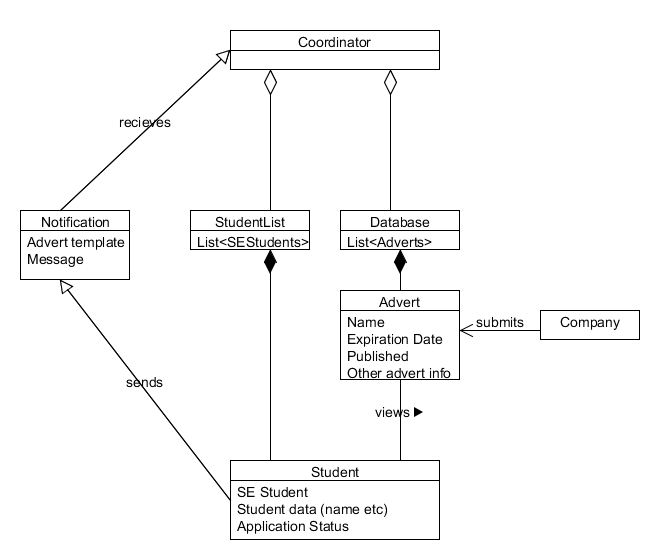
\includegraphics[scale=0.75]{DomainModel.png}
  %\includegraphics[width=60mm]{myfig.png}
  %\includegraphics[height=60mm]{myfig.jpg}
  %\includegraphics[angle=45,width=52mm]{myfig.jpg}

%%%%%%%%%%%%%%%%%%%%%%%%%%%%%%%%%%%%%%%%%%%%%%%%%%%%%%%%%%%%%%%%%%%%%%%%%%%%%%

\section{Use Case Descriptions}
This is a collection of use case descriptions (one per use case).
Think carefully about how to group these descriptions in the document.
You can use the template style provided to format your descriptions:

ADDED THIS TO CHECK


\begin{UseCaseTemplate}
\UseCaseLabel{Student Logs into system}
\UseCaseDescription{A student from the University of Glasgow
  interested in applying for a summer placement/internship gains
  access to the system by logging in.}
\UseCaseRationale{A student should be able to log into the
  system. This gives the system added protection and privacy to those
  who should not have access to the system.}
\UseCasePriority{High}
\UseCaseStatus{Uncomplete}
\UseCaseActors{Student}
\UseCaseExtensions{}
\UseCaseIncludes{}
\UseCaseConditions{}
\UseCaseNonFunctionalRequirements{}
\UseCaseScenarios{Successful log in, Unsuccessful log in.}
\UseCaseRisks{Unable to link with GUID log in which may mean students
  have to enrol for service. }
\UseCaseUserInterface{Log in screen.}
\end{UseCaseTemplate}

\begin{UseCaseTemplate}
\UseCaseLabel{Notification of new placement}
\UseCaseDescription{When a new placement is accepted by the course
  coordinator, all student in Level 3 CS should be notified of it by 
  email.}
\UseCaseRationale{A useful feature to aid CS students in their search
  for a placement}
\UseCasePriority{Medium}
\UseCaseStatus{Uncomplete}
\UseCaseActors{Student, Course Coordinator}
\UseCaseExtensions{}
\UseCaseIncludes{}
\UseCaseConditions{}
\UseCaseNonFunctionalRequirements{}
\UseCaseScenarios{Notification Sent}
\UseCaseRisks{Handeling the response from an email being sent to a 
  non-existent email address or to an email address that causes a 
  bounceback/send fail message. A student neglecting to view emails
  sent by the service due to mass emails sent when many advertisements
  go live on one day.}
\UseCaseUserInterface{Course Coordinator Advert View Screen.}
\end{UseCaseTemplate}

\begin{UseCaseTemplate}
\UseCaseLabel{}
\UseCaseDescription{}
\UseCaseRationale{}
\UseCasePriority{}
\UseCaseStatus{}
\UseCaseActors{}
\UseCaseExtensions{}
\UseCaseIncludes{}
\UseCaseConditions{}
\UseCaseNonFunctionalRequirements{}
\UseCaseScenarios{}
\UseCaseRisks{}
\UseCaseUserInterface{}
\end{UseCaseTemplate}


%%%%%%%%%%%%%%%%%%%%%%%%%%%%%%%%%%%%%%%%%%%%%%%%%%%%%%%%%%%%%%%%%%%%%%%%%%%%%%

\section{Non Functional Requirements}

The system can be accessed from anywhere with an internet connection and a
browser. The only authentication required is the staff or student's GUID or 
the company's login.

The systems availability should be continual with no unplanned downtime
throughout the calendar year. Adding and removing adverts, changing user status,
and any other specific functionality of the system should not require downtime
for the updating of any associated databases. Changes should be instantaneous,
in similar respects to an internet forum. There may be maintenance required on
the system to fix any errors but this should be at most one hour per week.

Only University of Glasgow students can access the advertisements. This is 
further limited to students registered with the School of Computing Science. 
Companies wishing to submit advertisements are given separate logins at the 
discretion of the Course Coordinator.

The mass email system will not impact on the continuing functionality of the 
application and viewing system for the Course Coordinator who should be able 
to complete other tasks while this is in operation.

The overall number of concurrent users on the system is dependant on the 
systems infrastructure and should not have a capped user limit.


%%%%%%%%%%%%%%%%%%%%%%%%%%%%%%%%%%%%%%%%%%%%%%%%%%%%%%%%%%%%%%%%%%%%%%%%%%%%%%

\section{Summary}

The system, in summary, is to allow companies to submit internship
advertisements for review by the Course Coordinator (CC). The CC either 
allows the advert in its current form and publishes it for students to view
or contacts the company out with the system with their comments on how to
improve the advertisement. Students view the advertisements and apply for
the internships they are interested in via the method stated in the
advertisement. Student's progress for obtaining an internship is tracked by
and controlled by the CC.

%%%%%%%%%%%%%%%%%%%%%%%%%%%%%%%%%%%%%%%%%%%%%%%%%%%%%%%%%%%%%%%%%%%%%%%%%%%%%%

\appendix

\section{Glossary}

\begin{itemize}

\item Course coordinator - A member of staff in the University of Glasgow's
School of Computing Science who is the sole administrator for the system and, as
a result, is responsible for reviewing advertisements and keeping track of 
student progress through the system.

\item CS - Computing Science

\item GUID - University of Glasgow user account held by all students and staff
members.

\item ESE - Electronic Software Engineering

\item SE - Software Engineering

\end{itemize}

%\section{Scenarios}

%A collection of scenarios you developed to exercise and refine your
%use cases.

\section{Stakeholder Interview Documentation}

The stakeholder interview conflicted with the requirements specification more
than it clarified. In addition to this, most questions that don't fall into the
former category were typically answered either by stating the specified
feature is out with the scope of the system or the interviewee did not
know the answer.

\section{Stakeholder Panel Documentation}

This section will list main points, in summary form, clarified in the
stakeholder panel. The information is not currently in any logical order.

\begin{itemize}

\item The advertisement submission screen will contain a standard form to
ensure companies submit required information such as duration of placement, and
wages. There will also be a text box to allow a company to submit any other
information they wish to provide.

\item For internships obtained out with the system, the student is to submit
a form to the Course Coordinator. The form is a reduced version of the
aforementioned advertisement submission form.

\item The system will have a single course coordinator whom will act as
the system administrator however this position can be reassigned.

\item An advertisement can be edited by the associated company prior to
publishing.

\item Deletion of advertisements can be executed manually by either the course
coordinator or associated company. This can be done when an internship placement
has been filled up or if a company wishes to amend an advertisement. Amendments
after publication require a deletion of the old advertisement since they are
frozen after publication.

\item University students and staff will use their GUID to login to the system
and companies will use separate accounts supplied by the course coordinator.
Any additional information, such as address and telephone numbers, can then
be obtained via the University's MyCampus system.

\item Via a dashboard, the course coordinator is able to view a summary of
students' statuses in the system. This can be used to contact students not
currently in an application process to remind them to apply to internships. The
course coordinator can download status information to a CSV file.

\item Recruitment agencies and other internship management systems, such as
Club 21, are treated in the same way companies are.

\item The University will already have a mailing list of CS/SE/ESE students
however, the system will not be using this. Instead the system will have its
own mailing list. A student will automatically be added to the mailing list
and can only be removed once a placement has been secured and approved.
Notification of new internships via this mailing list can be sent in a variety
of frequencies, including: instantaneously; daily; bi-weekly etcetera.

\item The stakeholder panel clarified an important point: who can view what
in the system. The course coordinator can be everything. The companies can see
their own advertisements. The students can see all published internships, even
if they have been marked as unsuitable for the student's degree.

\end{itemize}

%%%%%%%%%%%%%%%%%%%%%%%%%%%%%%%%%%%%%%%%%%%%%%%%%%%%%%%%%%%%%%%%%%%%%%%%%%%%%%

\end{document}

%%%%%%%%%%%%%%%%%%%%%%%%%%%%%%%%%%%%%%%%%%%%%%%%%%%%%%%%%%%%%%%%%%%%%%%%%%%%%%
